\chapter*{Kurzfassung /Abstract }
\label{cha:abstract}

Die vorliegende Diplomarbeit beschäftigt sich mit subtraktiver Klangsynthese mittels elektronischer Hardware am Beispiel eines selbstgebauten modularen Synthesizers. \\

Der dokumentierte Synthesizer stellt ein in sich geschlossenes System dar, welches jedoch bei Bedarf mit externen Komponenten erweitert werden kann. Zu diesem Zweck streben wir Kompatibilität mit dem Eurorack-Format an, welches einen De-facto-Standard für modulare elektronische Synthesizer darstellt. \\ \\

This thesis deals with analog sound synthesis through electronic hardware using the example of a home-made modular synthesizer system. \\

The documented Synthesizer is a self-contained system, which can be extended by external components. To this end, we strive for compatibility with the eurorack format, which represents a de-facto standard for modular electronic synthesizer systems. \\

\newpage

\subparagraph{Projektergebnis}
Alle nötigen Module für eine klassische Signalverarbeitungskette zur subtraktiven Klangsynthese wurden recherchiert, entworfen und gefertigt. Das System entspricht wie geplant den Standards des Eurorack-Formates und ist somit mit einer Vielzahl von kommerziell erhätlichen Komponenten erweiterbar. Genauere Ausführungen zu den erreichten Zielen befinden sich im Schlussteil (siehe Abschnitt \ref{goals}).

\subparagraph{Result}
All necessary Modules to make up a standard signal processing chain for subtractive sound synthesis have been researched, designed and manufactured. As planned, the system conforms to the standards of the eurorack-formats and can therefore be expanded with a wide range of commercially available components. More detailed explanations of the achieved goals can be found in the final section (see chapter \ref{goals})

\begin{figure}[hb]
  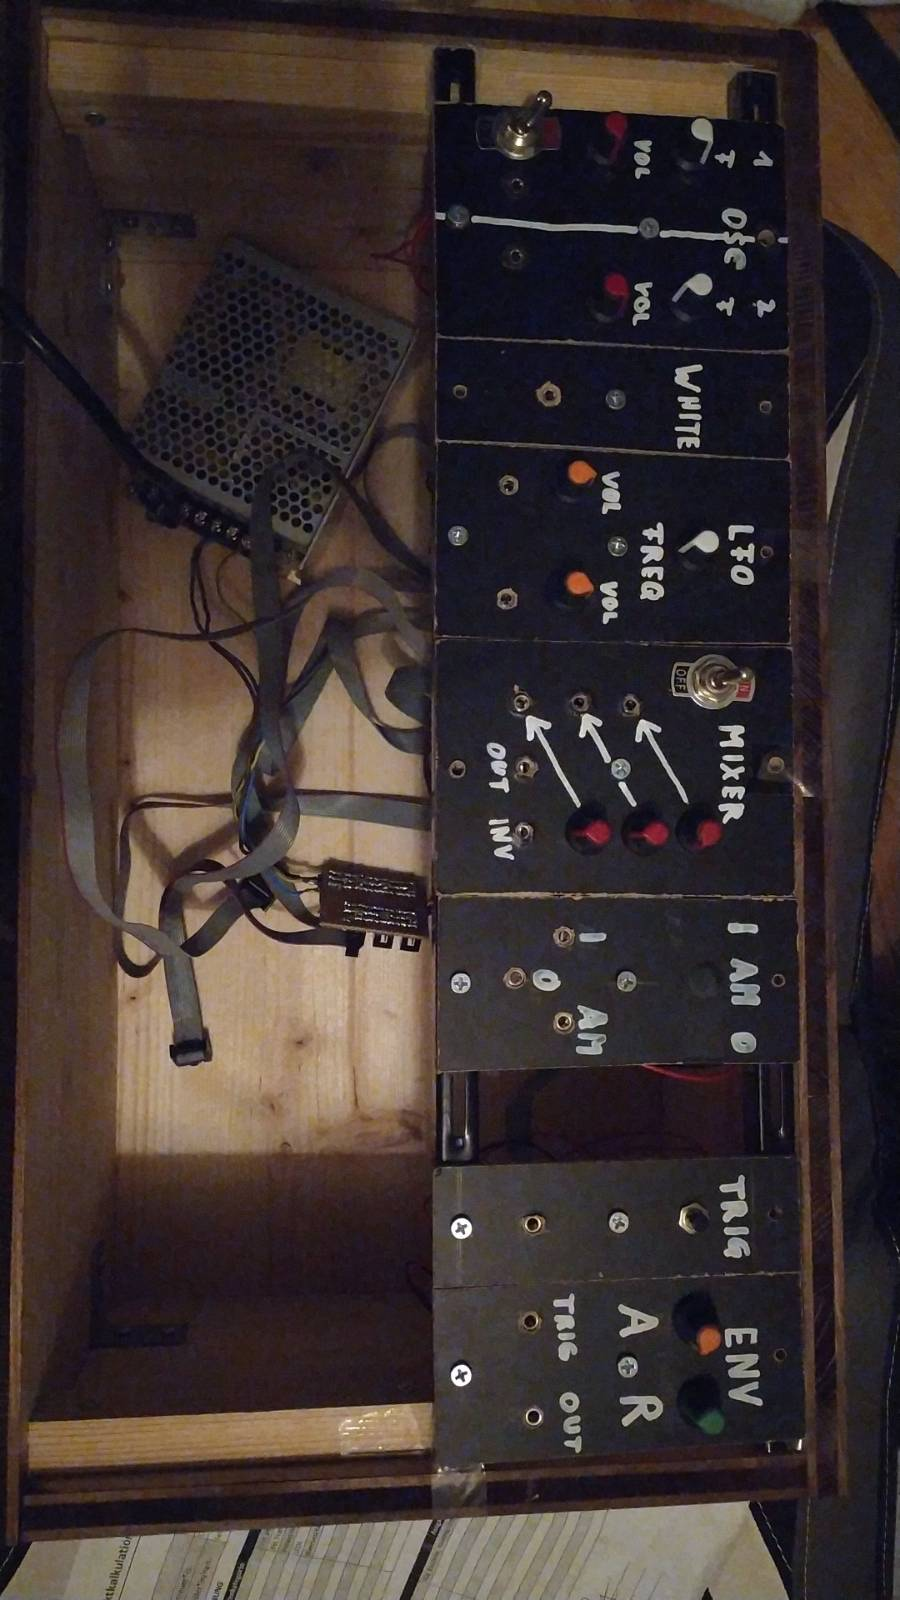
\includegraphics[angle=90,width=\linewidth]{figures/case.jpg}
  \caption{Der fertiggestellte Synthesizer mit allen Modulen, Spannungsquelle und Gehäuse}
  \label{fig:case}
\end{figure}
